\documentclass[meta,authordate,issue]{jote-new-article}
%\usepackage[top=0.85in,left=1.75in,footskip=0.75in,marginparwidth=2in]{geometry}

% Keyword commands
\providecommand{\keywords}[1]
{
  \small	
  \textbf{\textit{Keywords---}} #1
}

% use Unicode characters - try changing the option if you run into troubles with special characters (e.g. umlauts)
%\usepackage[utf8]{inputenc}
%\usepackage[most]{tcolorbox}

% clean citations
%\usepackage{cite}
%\usepackage{natbib}
\usepackage{amssymb}
\usepackage{amsmath}

% hyperref makes references clicky. use \url{www.example.com} or \href{www.example.com}{description} to add a clicky url
\usepackage{nameref,}

% line numbers
%\usepackage[right]{lineno}

% improves typesetting in LaTeX
%\usepackage{microtype}
%\DisableLigatures[f]{encoding = *, family = * }

% text layout - change as needed
%\raggedright
%\setlength{\parindent}{0.5cm}
%\textwidth 5.25in 
%\textheight 8.75in

\jissue{1}
\jvolume{4}
\jpages{73--81}
\paperissued{May 24, 2024}

\articletype{Special Issue - Meta Research}
\specialissue{Consequences of the Science Reform Movementt - \url{https://doi.org/10.36850/jote.i4.1}}

\setcounter{page}{73}

\addbibresource{library.bib}
% Remove % for double line spacing
%\usepackage{setspace} 
%\doublespacing

% use adjustwidth environment to exceed text width (see examples in text)
%\usepackage{changepage}

% adjust caption style
%\usepackage[aboveskip=1pt,labelfont=bf,labelsep=period,singlelinecheck=off]{caption}

% remove brackets from references
% \makeatletter
% \renewcommand{\@biblabel}[1]{\quad#1.}
% \makeatother

% headrule, footrule and page numbers
\usepackage{lastpage}
\usepackage{epstopdf}
% \pagestyle{myheadings}
% \pagestyle{fancy}
% \fancyhf{}
% \rfoot{\thepage/\pageref{LastPage}}
% \renewcommand{\footrule}{\hrule height 2pt \vspace{2mm}}
% \fancyheadoffset[L]{2.25in}
% \fancyfootoffset[L]{2.25in}

% use \textcolor{color}{text} for colored text (e.g. highlight to-do areas)
%\usepackage{color}

% define custom colors (this one is for figure captions)
\definecolor{Gray}{gray}{.25}

% this is required to include graphics
%\usepackage{graphicx}

% use if you want to put caption to the side of the figure - see example in text
\usepackage{sidecap}

% use for have text wrap around figures
\usepackage{wrapfig}
\usepackage[pscoord]{eso-pic}
% \usepackage[fulladjust]{marginnote}
% \reversemarginpar

% \usepackage{xpatch}

%%%%%%%%%%% Defining Enunciations  %%%%%%%%%%%
% \newtheorem{corollary}{\bf Corollary}[section]
% \newtheorem{theorem}{\bf Theorem}[section]
\newtheorem{condition}{\bf Condition}[section]
%%%%%%%%%%%%%%%%%%%%%%%%%%%%%%%%%%%%%%%%%%%%%%%

%%%%%%%%%%% User Defined  Commands  %%%%%%%%%%%
\newcommand{\X}{\mathbf{X}}
\newcommand{\Y}{\mathbf{Y}}
\newcommand{\Z}{\mathbf{Z}}
\newcommand{\W}{\mathbf{W}}
\newcommand{\E}{\mathbb{E}}
%
\definecolor{myred}{RGB}{192, 0, 17}
% \usepackage[inline]{trackchanges}
%  \addeditor{E}
%  \addeditor{B}
%  \addeditor{D}
\let\tinyurl\url
%---------------------------------------------------------
% Colored text box, user defined
\newtcolorbox{mybox}[1][]{%
    colback=black!5,
    colframe=black!5,
    notitle,
    sharp corners,
    borderline west={1pt}{0pt}{black!80!black},
        borderline east={1pt}{0pt}{black!80!black},
            borderline north={1pt}{0pt}{black!80!black},
                borderline south={1pt}{0pt}{black!80!black},
    enhanced,
    breakable,
    }
    
% \newcounter{definition}
% \newenvironment{definition}[1][]{\refstepcounter{definition}\par\medskip
%    \noindent\textbf{Definition~\thedefinition. #1} \rmfamily}{\medskip}
   
\newcounter{result}
\newenvironment{result}[1][]{\refstepcounter{result}\par\medskip
   \noindent\textbf{Result~\theresult. #1} \rmfamily}{\medskip}

% \newcounter{remark}
% \newenvironment{remark}[1][]{\refstepcounter{remark}\par\medskip
%    \noindent\textbf{Remark~\theremark. #1} \rmfamily}{\medskip}

   \jotetitle{Tension Between Theory and Practice of Replication}
   \keywordsabstract{formal theory, scientific reform, reproducibility, replication, multi-site replications, \mbox{meta-hypothesis}}
   \abstracttext{A core problem that has been addressed in the scientific reform movement so far is the low rates of reproducibility of research results. Mainstream reform literature has aimed at increasing reproducibility rates by implementing procedural changes in research practice and scientific policy. At the sidelines of reform, theoreticians have worked on understanding the underlying causes of irreproducibility from the ground up. Each approach faces its own challenges. While the mainstream focus on swift practical changes has not been buttressed by sound theoretical arguments, theoretical work is slow and initially is only capable of answering questions in idealized setups, removed from real life constraints. In this article, we continue to develop theoretical foundations in understanding non-exact replications and meta-hypothesis tests in multi-site replication studies, juxtapose these theoretical intuitions with practical reform examples, and expose challenges we face. In our estimation, a major challenge in the next generation of the reform movement is to bridge the gap between theoretical knowledge and practical advancements.}
   \runningauthor{Buzbas \& Devezer}
   \jname{Journal of Trial \& Error}
   \jyear{2023}
   \paperpublisheddate{2023-11-02}
   \paperdoi{10.36850/mr9}
   \paperreceived{November 28, 2022}
   \author[1,*]{Erkan Buzbas}

   \affil[*]{Both authors contributed equally to this work.}
   \affil[1]{Department of Mathematics and Statistical Science, University of Idaho}
   \corraddress{University of Idaho, Department of Business}
   \author[1,2,*]{Berna Devezer\orcid{0000-0002-5979-2781}}
   \corremail{\href{mailto:bdevezer@uidaho.edu}{bdevezer@uidaho.edu}}
   \affil[2]{Department of Business, University of Idaho}
   \funding{Research reported in this publication was supported by the National Institute Of General Medical Sciences of the National Institutes of Health under Award Number P20GM104420. The content is solely the responsibility of the authors and does not necessarily represent the official views of the National Institutes of Health.}

   \paperaccepted{August 22, 2023}
   \paperpublished{November 2, 2023}
   \jwebsite{https://journal.trialanderror.org}

% \@addtoreset{section}{part}
%---------------------------------------------------    
% document begins here
\begin{document}
\pdfbookmark[0]{Buzbas \& Devezer (2023). Tension Between Theory and Practice of Replication}{3}
\begin{frontmatter}
  \maketitle
  \begin{abstract}
    \printabstracttext
  \end{abstract}

\end{frontmatter}

% title goes here:
% \begin{flushleft}
%   {\Large \textbf\newline{Tension between theory and practice of replication}}
%   % Bridging the gap between formal theory and scientific reform practices
%   \newline
%   % authors go here:
%   \\
%   Erkan Buzbas \textsuperscript{1\ddag},
%   Berna Devezer \textsuperscript{1,2*\ddag }
%   \\
%   \bigskip
%   \bf{1}Department of Mathematics and Statistical Science, University of Idaho
%   \\
%   \bf{2}Department of Business, University of Idaho
%   \\
%   \bigskip
%   *Corresponding author (bdevezer@uidaho.edu)\\
%   \ddag The authors contributed equally to this work.\\


% \end{flushleft}

% NEED TO INCLUDE THE FOLLOWING
%\keywords{Formal theory, Scientific reform, Reproducibility, Replication, multi-site replications, Meta-hypothesis}
% \corres{Berna Devezer\\
% \email{bdevezer@uidaho.edu}}

\lettrine{T}{he} scientific reform movement that was propelled by exposing a scientific replication crisis has attracted interest of scholars spanning a wide range of disciplines from social and biomedical sciences to humanities and formal sciences. A core problem attacked has been low rates of results reproducibility\footnote{Also referred to as \textit{replicability} in the literature.} (given a result from an original study, the probability of obtaining the same result in replication experiments) in some scientific disciplines. We have argued elsewhere that first generation approaches have predominantly aimed at reforming scientific policy and practice to improve results reproducibility, at times based on hasty diagnoses of problems and normative implementations of procedural solutions~\parencite{Devezer2021}. This approach of reforming scientific practices via bureaucratic innovations~\parencite{Penders2022} has effectively, if unintentionally, derailed the investigation of underlying causes of results reproducibility and deprioritized a rigorous theoretical foundation. We fear that this may have led to the illusion that fundamentally mathematical, complex issues can be solved with procedural fixes. Perhaps such mechanistic solutions may indeed help improve the efficiency of certain scientific processes~\parencite{Peterson2023}. But if we aim to address mathematical problems, the ability to identify and attack them as mathematical seems critical. For example, it should be clear that the true reproducibility rate of a true result in a sequence of exact replication studies with independent and identically distributed random samples  can take any value on $[0,1]$ depending on the elements defining that study. Thus, we should not have a default expectation of high rates of reproducibility or assume that low reproducibility is indicative of false discoveries~\parencite{Buzbas2023}. A designation of {\em crisis} could as well point to a problem with our expectations. How do we calibrate our expectations from replication studies, especially regarding reproducibility rates?

As statisticians, explanations and solutions that we deem satisfactory for a procedure require clear and precise reporting about models and analyses. In contrast, many high-profile, multi-site replication studies reporting on results reproducibility fail to even state the statistical model under which inference is made~\parencites[e.g.,][]{klein2018many}{open2015estimating}. We would be in a precarious position to interpret any results or make statistical recommendations without providing a statistical model and tight theoretical reasoning for it. Such precision is not trivial or merely decorative. As many analyst studies~\parencites{breznau2022observing}{Silberzahn2018} show with striking clarity, our inference depends on and may drastically vary with the statistical models we assume.

On the other hand, precision is useless without theoretical understanding. As John von Neumann said: ``There's no sense in being precise when you don't even know what you're talking about.'' So not only do we need precise reporting of model specification but also a statistical understanding of its assumptions, performance, and implications. In this sense, there is a growing tension between the practical and theoretical foci in science reform, and from a theoretical perspective, there is a lot of room for improvement with regard to the rigor of statistical reasoning in the first generation reform literature. Such theoretical reasoning stands to provide much needed clarity and precision in making sense of the practical advances the reform movement has brought about. However, there are outstanding challenges on the theory side of things as well.

In this article, we aim to provide insight into the process of thinking about some key statistical issues regarding the reproducibility of scientific results, particularly in current big team applications of multi-site replication studies. We strive to expose what it takes to make precise statistical statements, what kind of questions are raised and need to be addressed on the way, and why this matters. Key points of theoretical exposition are the importance of distinguishing between exact and non-exact replications, and their proper statistical treatment in the analyses of replication data. We believe that a strong theoretical understanding of non-exact replications should inform our interpretation of results reproducibility in replication studies. We further evaluate the consequences of this distinction on testing meta-hypotheses in large-scale multi-site replication studies using well-established statistical theory. Our treatment will hopefully make clear what exactly can be gained by stronger theoretical foundations in science reform moving forward. Finally, as a next generation challenge, we propose the daunting yet necessary interdisciplinary work of bringing the theory and practice closer together.

\section{Distinguishing between exact and non-exact replications}

We set out to work with an idealized version of the real-life problem regarding the divergences between replication studies and the originals. An idealized study comprises background knowledge, an assumed statistical model, and statistical methods to analyze a sample, which is  generated under the true model independent of all else~\parencite{Devezer2021}. A {\em result} is a function from the space of analysis to the real line. To evaluate the reproducibility rate of a result obtained from a sequence of studies, all replications must randomly sample the same sampling distribution of results. This is guaranteed if a sequence of replication studies are {\em exact} replications, that is, only the random sample is new across the replications. Statistically, the best way to assess whether a given result from one study is reproduced in its replications is by the relative frequency of that result in all replication studies. A major value of this idealization is advancing understanding of the theory of results reproducibility under exact replications.

In practice, this idealized setup is unrealistic, given uncontrollable sources of variability across replications. No sensible person would argue that they have replicated another study exactly, except perhaps under rare, extremely well-controlled studies. The main issue is that we expect the natural phenomenon represented to be distorted by specific conditions contributing to the design in different ways because every controlled study imposes constraints of its own. Some concrete evidence showing this comes from purpose-built and performed large-scale replication studies. These studies have not been able to fix the design parameters so as to perform exact replication studies of each other. Examples of variations in study parameters purported to be replications of each other may include:
\newpage
\begin{itemize}
  \item studies sampling only subsets of populations (i.e., non-random sampling of a larger population),
  \item unequal sample sizes,
  \item missing data of different kinds,
  \item differences in sampling methods,
  \item differences in post-processing of data,
  \item differences in statistical analysis methods.
\end{itemize}
Therefore, with the exception of specialized studies where extremely well-controlled designs involving few random variables can be implemented---such as in particle physics---we argue that exact replication experiments are unlikely to be operationalized in daily science. Consequently, the sampling distribution of the results in replication studies will differ from that of the original study or from each other, and drawing conclusions about result reproducibility becomes a challenging problem. Leaving aside the (perhaps more important) issue of why the sampling distributions differ from each other, how they differ from each other becomes the primary objective to understand if we are to study results reproducibility properly. Hand-waving at a sequence of non-exact replications as ``conceptual replications'' and claiming to test the generalizability of an underlying effect won't do as it is begging the question. Therefore, to develop a broad theory of results reproducibility, we must work with a sequence of not-necessarily-exact replications, and treat the case of exact replications as a special case.

Unfortunately, for non-exact replications, we have very limited theory. What we know  can be summarized as follows. A sequence of replication studies can be treated as a proper stochastic process. If all the elements of replication studies are exactly equivalent to each other except the sample generated under the true model, then the case of exact replications can be treated as a special case, yielding a single sampling distribution of reproducibility rate. When replications are non-exact, there is no single true reproducibility rate for results from all studies and therefore, no single sampling distribution of reproducibility rate. The mean of the process, then, becomes the target, but it needs to be interpreted carefully~\parencite[see][for more information]{Buzbas2023}.

A critical matter is that theoretical conclusions about reproducibility depend on the choice of the {\em result}, and hence the mode of statistical inference in studying results reproducibility. Harking back to L. J. Savage, we believe that the {\em result} needs to be ``as big as an elephant'' to allow for generalizability of conclusions. The least useful mode of statistical inference to study results reproducibility is the null hypothesis significance test under the frequentist approach due to its inflexible interpretation of results probabilistically (e.g., cannot talk about probability of a result unconditional of a hypothesis) and its forced dichotomization of results in hypothesis testing (e.g., reject or fail to reject). These properties obscure the measurable quantitative signal in studies of reproducibility, thereby decreasing the resolution in results which could be used to understand the mechanisms driving irreproducibility. If there exists a problem of result reproducibility in hypothesis testing, it will likely exist under other major modes of inference such as point estimation, interval estimation, model selection, and prediction of future observables.

An efficient way to investigate results reproducibility information theoretically is under a more mathematically refined mode of inference than null hypothesis significance testing. Estimation theory is the best understood mode of statistical inference, equipped with most well-established theorems. It is our safety net. Based on estimation theory, model selection is a challenging but ultimate target in modern statistics~\parencite[as well as in][]{Devezer2019}.

Now that we have laid out our foundations, let us turn to the theoretical challenges that arise when trying to understand results reproducibility from non-exact replications.

\section{Evaluating the results from non-exact replications with respect to results reproducibility}

In this section we discuss the problem of evaluating results reproducibility from replication studies. Our perspective involves reference to the true data generating mechanism $M_T,$ which we assume exists and we would like to operate under\footnote{If $M_T$ does not exist, we chase a moving target. There are some tools of mathematical statistics to study these cases (see for example  M-open versus M-closed discussion in \cite{bernardosmith2000} and references therein), but these are out of our scope for the treatment of results reproducibility.}. For convenience and purposes of illustration, we assume a linear model with additive errors $M_T:= \; \{Y|\X_T\beta_T = \X_T\beta_T+\epsilon\},$
which is well-studied and accommodates common research studies. Here, $Y$ is $n \times 1$ vector of response variables, $\X_T$ is $n \times p$ matrix of predictors (e.g., design matrix in experiments), $\beta_T$ is $p \times 1$ vector of model parameters, and $\epsilon$ is $n \times 1$ vector of stochastic errors. It is convenient to assume zero mean, constant variance, and uncorrelated errors, which are collectively known as the ordinary least squares (OLS) assumptions. Often, a full model specification is required for analysis, so these assumptions are augmented with normal distribution of errors. Thus, $M_T$ is an exactly determined representation of a natural phenomenon of our interest or in other words, the {\em target true} data generating mechanism. In practice, we may not know the space on which $M_T$ exists. It is worth mentioning that only if the set of models considered by a researcher includes $M_T,$ we can hope to study results reproducibility of true results. More precisely, we should be able to include $M_T$ in our consideration of data generating mechanisms with possible null values for some parameters. Here, we assume that we can satisfy this assumption. However, we invite the reader to ponder how challenging it is to satisfy this assumption in practice. For the discussion below, we also define $M_O,$ the assumed model in the original (first) study, and $M_R,$ the assumed model in a subsequent replication study.

Hypothetically, in an ideal study there should be no {\em intervention by the study} which distorts the data generated by $M_T.$ If the study assumes that it is operating under $M_T$ as the data generating mechanism, the model is correctly specified and the solution $\hat{\beta}_{T}= (\X_{T}^{'}\X_{T})^{-1}\X_{T}^{'} Y$ are best linear unbiased estimators. Almost all statistical inferential goals require some version of $\hat{beta}_T$ under linear models. Therefore, without loss of generality, here we set it as an example of a target {\em result}.

We believe that the hypothetical scenario of no intervention by a study is not realistic to evaluate results reproducibility from a sequence of studies because it requires the equivalence of $M_T,\;M_O\;,M_R,$ and so on for other replication studies. This equivalence means that all variables that are indeed in $M_T$ are included in $M_O$ and $M_R,$ and no variable that is not in $M_T$ are excluded in $M_O$ and $M_R$\footnote{Note that we have already made the simplifying assumption of operating in a universe of linear models. In reality, the functional form of the relationship among variables is another factor that can vary across $M_T,\;M_O\;,M_R$.}. Again, in practice any study introduces its constraints on the data generating mechanism---see the list in the preceding section for some examples of constraints. If we proceed on this assumption, then $M_O$ is likely not equivalent to $M_T.$ So we ask: In which aspects $M_O$ differ from $M_T?$ Naturally, we also ask: In which aspects $M_R$ differ from $M_O$?

A reviewer has raised the question of why $M_T$ needs to be invoked at all to compare results reproducibility from $M_O$ and $M_R,$ since they do not involve $M_T$ directly, with good reason. That is, it is sufficient to assess whether $M_O$ and $M_R$ are equivalent without reference to $M_T$. This assessment is fair but it invites further difficulties of statistics to the study of results reproducibility. $M_O$ equivalent to $M_R$ but not equivalent to $M_T$ is the case of inference from replications under {\em model misspecification}. We defer discussing some of the issues related to this case to the end of this section drawing from a broader lore of mathematical statistics. In the next paragraph, we briefly focus on the consequences of all three models being different from each other on estimates.

We assume that the original study includes only some of the variables that are indeed in $M_T,$ and also includes some variables that are not part of $M_T$ in the assumed model. The relevant matrix of predictors (e.g., design matrix) which we denote by $\X_{O}$ in the assumed model $M_O$ has now changed. If it is correctly identified, this study operates under the data generating model
%
$M_O:=\; \{Y|\X_{O}\beta_{O} = \X_{O}\beta_{O}+\epsilon\},$
%
and the solution for OLS estimates in $M_O$ is now
$\hat{\beta}_{O}= (\X_{O}^{'}\X_{O})^{-1}\X_{O}^{'} Y.$
%
There is no convincing argument to assume that $M_O$ is equivalent to $M_T.$ Thus, $\beta_{T} \neq \beta_{O}$ implying that $\hat{\beta}_{T} \neq \hat{\beta}_{O}$ given the same data. Even if $M_O$ is equivalent to $M_T,$ it is more likely for the replication studies in the sequence to generate data under models different than $M_T$ or $M_O$ via the process of inclusion and exclusion of variables and due to examples of variations listed in the previous section. Let the assumed model (if identified correctly) in a replication study be
%
$M_R:=\; \{Y|\X_{R}\beta_{R} =\X_{R}\beta_{R}+\epsilon\},
$
%
and the solution for OLS estimates in $M_R$ is now
$\hat{\beta}_{R}= (\X_{R}^{'}\X_{R})^{-1}\X_{R}^{'} Y.$
%
%
Thus, $\hat{\beta}_{T}, \hat{\beta}_{O},$ and $\hat{\beta}_{R}$ are not equivalent estimates even when they see the same data.

For the case where $M_O$ and $M_R$ are equivalent to each other but different from $M_T,$ we would have $\hat{\beta}_{O}=\hat{\beta}_{R},$ and we can assess the reproducibility rate of a specific result since we have exact replications. Assuming the number of studies all under $M_O$ increases, the estimated reproducibility rate converges to the true reproducibility rate of the specific result. The problem with this rate is that it is the true reproducibility rate of a false or true result obtained under the misspecified model $M_O.$ There is no systematic approach that can tell how the misspecification affects the truth or falsity of the obtained result. That is, even if we assume that $M_O$ is close enough to $M_T$ to pass, say a pre-determined criterion model-wise, we do not have a theory that would guarantee that the reproducibility rate of a specific (true) result obtained under $M_O$ would be close to the reproducibility rate of the same type of result obtained under $M_T.$ The closeness of the models does not guarantee the closeness of the reproducibility rates of all results and the relationship is often a function of the result and the type of the model misspecification itself. In other words, we cannot tell what rate of reproducibility to expect for a given result under model misspecification unless we study the particular kind of misspecification in a given context. Nor can we tell what a successful or failed replication means exactly. If, however, a theory of dependence between reproducibility rate of results under correctly specified models and misspecified models can be built, then the condition of direct equivalence of $M_T$ and $M_O$ can be bypassed. Building such a theory would require measuring the discrepancy between $M_T$ and $M_O$ which still requires knowledge of $M_T$ to some extent. The consequences of model misspecification are often case specific, and strong results for broad classes of models have been elusive to frustration of statisticians. This issue is beyond the scope of this paper and by invoking $M_T$ as our target, we believe that we can have a more fruitful first step in discussing results reproducibility, at least at this early theoretical stage of the field.



\newpage
\subsection{A simple example to show drastic effects of non-exact replications}

Let us assume that the true model is $M_T:=E(Y|\beta_{T})=\beta_{T},$ that is a one-parameter model with no predictors. Our interest is to estimate the population mean $\beta_{T}$ using the sample $Y_1,Y_2,\cdots, Y_n$ independently generated under the assumed model in the original study $M_O:=E(Y|\beta_{O})=\beta_{O}.$ As we have indicated in general $\beta_{O} \neq \beta_{T}.$ Without loss of generality, let us define a very simple relationship $\beta_{O}=\beta_{T}+c,$ where $c\neq 0$ is some constant. The best estimator of the population mean is the sample mean and so we use the estimator $\hat{\beta}=n^{-1}\Sigma_{i=1}^{n}Y_i.$ However, we quickly realize that $E(\hat{\beta})=E(Y|\beta_{O})=\beta_{O}=\beta_{T}+c.$ Thus, the sample mean obtained in the study with assumed model $M_O$ is a {\em biased estimator} for the true population mean of interest $\beta_{T}$ under the true model. And it gets worse. We also quickly realize that by weak law of large numbers $\hat{\beta}$ is a consistent estimator of $\beta_{O}$ the population mean from which the sample is drawn and  $\beta_{T}=\beta_{O}-c$ implies that the probability $P(|\hat{\beta}-\beta_{T}|>\delta)$ does not converge to $0$ for any small $\delta>0$ as the sample size increases. Thus, the sample mean of the data obtained in the study with assumed model $M_O$ is also an inconsistent estimator for the true population mean of interest $\beta_{T}$ under the true model.
%
An immediate implication of this argument is on the choice of sample size as the divergent factor between a true model, an original study, and its replications. To assess the reproducibility of a given result, the result must be obtained from studies with equal sample sizes across original and replication studies and identical methods must be applied to arrive to a result. Researchers in practice might be tempted to increase the sample size in a replication (e.g., for higher statistical power as a better standard to meet). However, larger sample sizes do not necessarily imply that true results will be more reproducible. To extend the theoretical example given above, we consider testing the true hypothesis $\beta_{T} = 0$ using intervals $\hat{\beta} \pm SE(\hat{\beta}),$ where ${SE}(\hat{\beta})$ is the standard error of the sampling distribution of $\hat{\beta}$. The reproducibility rate defined as the proportion of the number of true results to the number of total results in a sequence of studies decreases with larger sample sizes, converging to zero (Figure~\ref{fig:samplesize}). This leads to a dilemma: Do we strive to conduct very few replication studies but making them as exact as possible at a great expense of resources because we know how to interpret their results theoretically, or do we try and run studies that are non-exact even if we do not quite understand what the implications of this non-exactness may be?

\begin{figure*}[b]
  \begin{fullwidth}
    \centering
    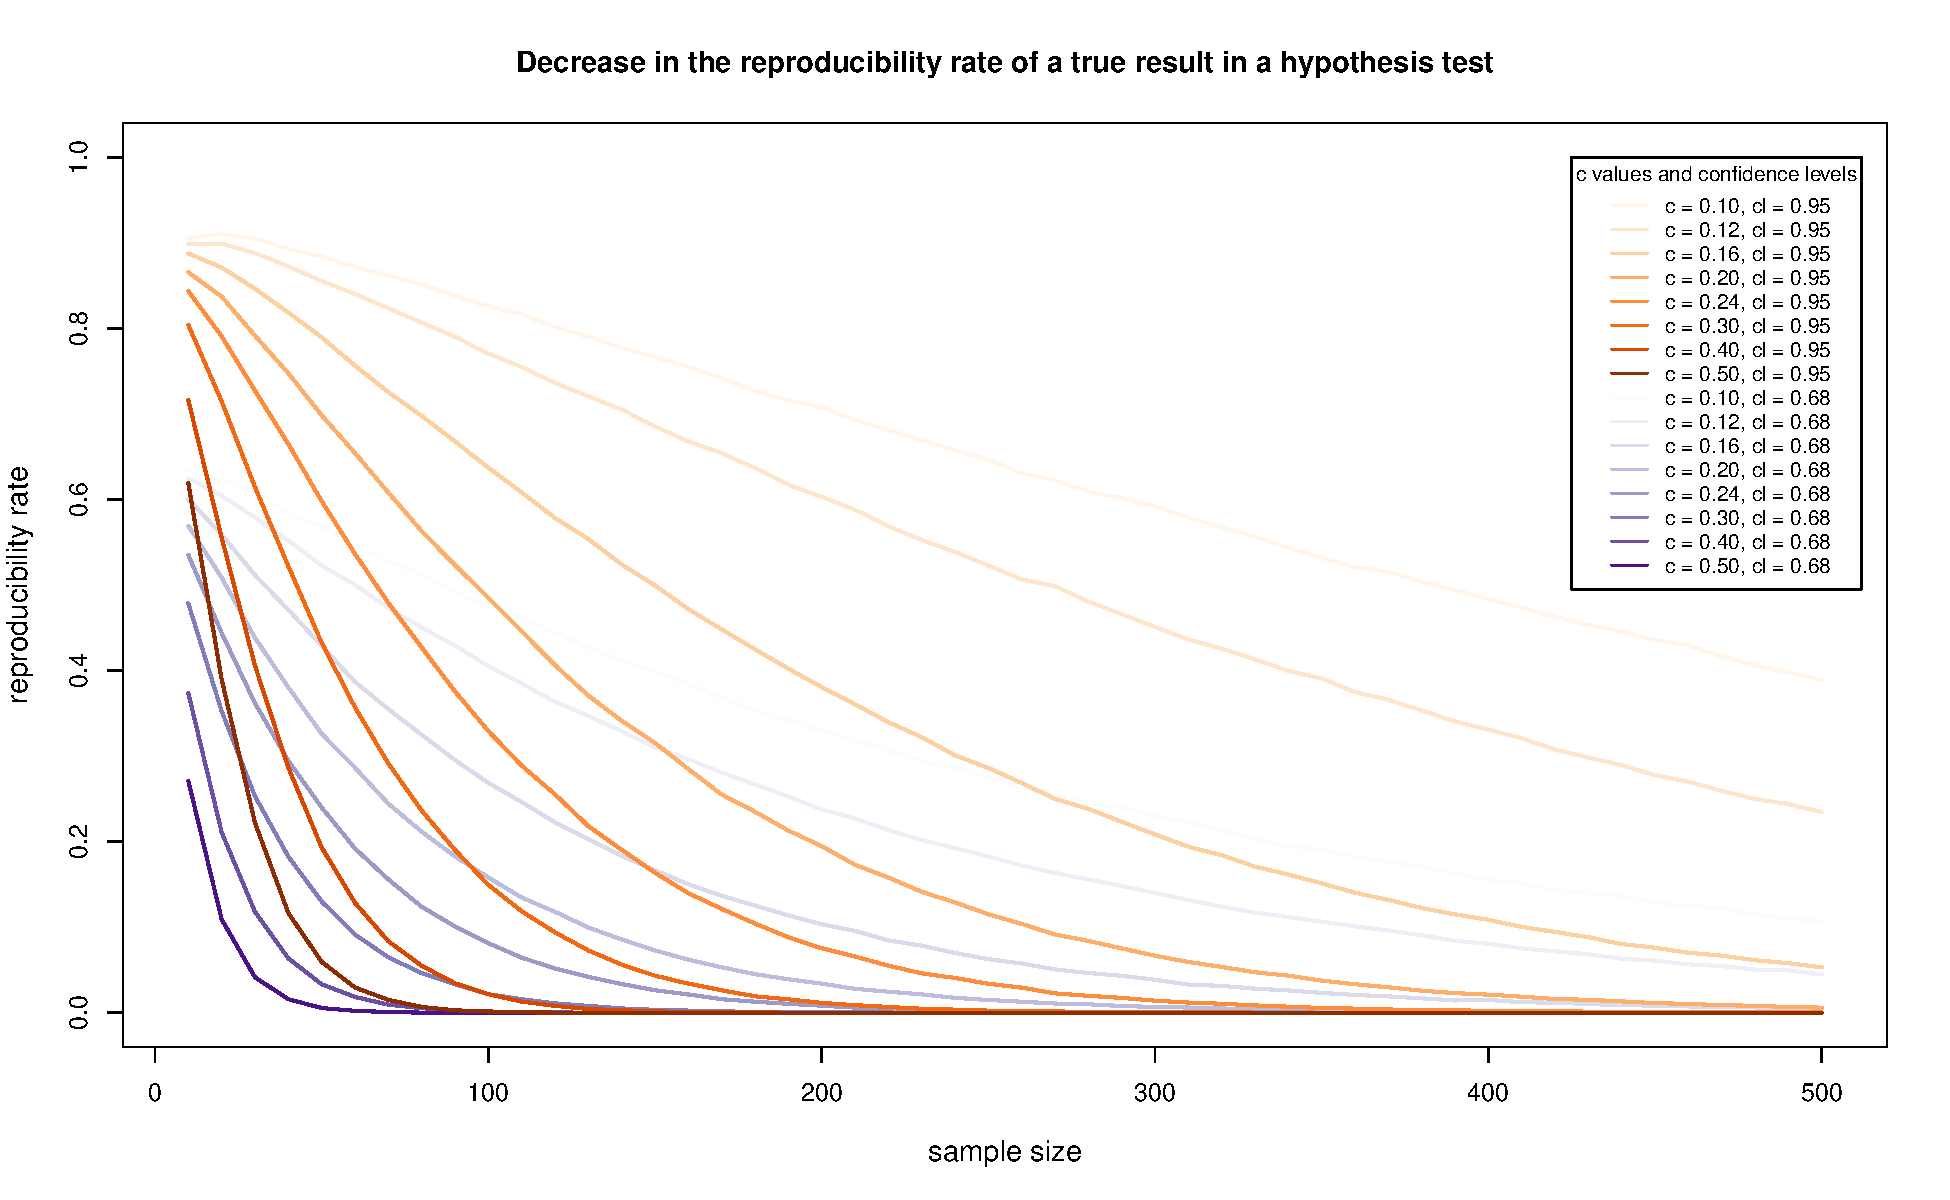
\includegraphics[width=\textwidth]{Figure_1.pdf}
    \caption{The reproducibility rate of a true result in a hypothesis test decreasing with increasing sample size. The (true) null hypothesis is $\beta_{T}=0,$ where $\beta_{O}=\beta_{T}+c$ and $c>0$  is a constant.}
    \label{fig:samplesize}
  \end{fullwidth}
\end{figure*}


We conclude that to connect the results of {\em non-exact} replication studies, we need theoretical results on how non-exact they are and what the exact effect of non-exactness is on the results. Once again, hand-waving at perceived closeness or likeness will further obscure our vision and make it more difficult to properly interpret the replication results. In~\textcite{Buzbas2023}, we show how easily true or false results can be made more or less reproducible with small perturbations in study design.

Many analyst studies~\parencites[e.g.,][]{breznau2022observing}{hoogeveen2022many}{Silberzahn2018} provide an example of how this type of non-exactness may play out in practice. In these studies, independent research teams are given the same data set and asked to perform analyses to test a given scientific hypothesis. What is striking is that not only inferential procedures but also assumed models vary greatly across analysts, resulting in a range of results not necessarily consistent with each other. Note that these studies use the same data set that samples a given population. In non-exact replication studies, inference is performed from independent data sets often sampling different populations. Also worth noting is that the many analyst results confirm our earlier point about the weakness of focusing on hypothesis tests instead of a more generic modeling framework.

\section{Studies for testing meta-hypotheses under non-exact replications}

As a more advanced example to show how the points we presented might affect the conclusions about results reproducibility in multi-site replication studies, we consider the following models for testing meta-hypotheses, in multi-site studies~\parencite[e.g., author involvement effect tested in Many Labs 4,][]{klein2022many}. For the $i$th observation, we define $g(u_i, v_i)$ as a function of $1 \times p$ vector of predictors such that $u$ are variables associated with the meta-hypothesis (e.g., varying on larger experimental units) and $v$ are variables associated with the original predictors (e.g., varying on smaller experimental units) of the study~\parencite{jones2009split}. The matrix of predictors $\X_{T^*}$ has $i$th row as $g(u_i, v_i).$ Due to two levels of the study, stochastic error must now conform not only the errors within each replication, but also the errors associated with meta-hypothesis. For the meta-hypothesis we have $\Z\eta$ where $\Z$ is $n \times k$ of indicator functions whose $k^{th}$ element is $1$ (e.g., for a level of meta-hypothesis) and others $0,$ and $\eta$ is $k \times 1$ vector of normally distributed errors with 0 mean and $\sigma_{\eta}^2$ variance. For replications we have $\epsilon$ is $n \times 1$ normally distributed errors with 0 mean and $\sigma_{\epsilon}^2$ variance for each observation. Assuming additive errors as before, we have $\Z\eta+\epsilon$ for stochastic errors, and $\eta_i$ and $\epsilon_j$ are assumed to be uncorrelated for all observation pairs $(i,j).$ The true model generating the data is
%
$M_{T^*}:=\; \{Y|\X_{T^*}\beta_{T^*} =\X_{T^*}\beta_{T^*}+\Z\eta+\epsilon\}.
$
%
Parallel to the argument leading to $M_O$ from $M_T,$
the {\em feasible generalized least squares estimates} in an original study $M_{O^*}$ is
%
$
  \hat{\beta}_{O^*} = (\X_{O^*}^{'}\widehat{\Sigma}^{-1}\X_{O^*})^{-1}\X_{O^*}^{'} \widehat{\Sigma}^{-1}Y,
$
%
where
$\Sigma=\sigma_{\eta}^2 \Z \Z^{'}+\sigma_{\epsilon}^2\mathbf{I}_{n}$
is the covariance matrix. $\Sigma$ is often unknown. It is estimated by sample variances at the meta-hypothesis and replication variables levels, assuming that the replications are exact.

The estimator $\hat{\beta}_{O^*}$ clearly shows why non-exactness of replications will exacerbate errors in estimates in larger models such as those used in testing meta-hypotheses. The reason is that larger models often require nuisance parameters also to be estimated in addition to parameters of interest. Even if we take the best approach to inference, the non-exactness of the replication will be reflected on multiple estimates resulting in undesirable estimators.

For our example, to obtain the estimate of interest $\hat{\beta}_{O^*},$ we also need to obtain
$\widehat{\Sigma}.$ The method of estimation for $\widehat{\Sigma}$ (e.g., restricted maximum likelihood or Bayes) will inevitably use $\X_{O^*}$ and the properties of $\widehat{\Sigma}$ will be affected by non-exactness of replications. This leads to biased estimates. Hence, non-exactness of replications casts more doubt on the inferential results of large models such as meta-hypothesis tests.

Many Labs 4~\parencite{klein2022many} provides a case study. The original hypothesis being tested over replications is the mortality salience effect and the experimental units are individual research participants; the meta-hypothesis being tested is the effect of original authors' involvement where experimental units are participating labs. The replications are non-exact in many ways from populations being sampled to unequal cell and sample sizes, from variations in in-house protocols to unequal block sizes. All of these factors likely bias effect size estimates in unpredictable ways. Considering the fact that inference is not made under a model that accounts for the randomization restriction and hierarchical experimental units in the actual experimental design, the results become even harder to interpret. The theory tells us what conclusions cannot be supported by the design and the analysis but it does not tell us what conclusions can be justified; that is, until that theory is advanced specifically for such cases.

\section{Conclusion}

We can clearly use mathematical statistics to advance our theoretical understanding of replications and results reproducibility under idealized conditions. This approach requires meticulous, persistent, and rigorous mathematical work that aims at theoretical clarity and precision. Nonetheless reality and scientific practice always impose new constraints on the problems at hand and as a result, oftentimes whenever theory meets reality, its reach falls short.

We know a lot about the consequences of exact replications yet we also know that exact replications are hard to achieve. In practice, we might think that even if we cannot perform exact replications, controlled lab conditions can approximate the ideal conditions assumed by statistical theory. This is a strong assumption that often gets violated. First, the effect of sampling different populations in replications cannot be remedied by randomization. Second, an approximation is a statement about a quantity approaching to another quantity in a precise mathematical way. It is not some haphazard likeness that we do not know how to define or verify. The mathematical approximation can be measured with precision but the perceived likeness of studies cannot. For example, for the sample mean, we know that the variance of its sampling distribution decreases with the inverse of the sample size linearly and we can measure the performance of this approximation in an analysis, data point per data point if need be. We would be challenged, however, to show how much a given replication study approximates an original study with respect to a reasonable measure in a statistical sense. The theory for measuring such closeness or likeness does not yet exist. Hence, our theoretical knowledge of exact replications is of little direct use for practice and for a thorough understanding of real life non-exact replications, we lack as rigorous a theory.




% One of the outstanding challenges for the second generation of scientific reform is to push the standards of transparency beyond preregistration and data sharing, to complete and precise specification of statistical models assumed and inferential procedures followed. There are several layers to this:
% \begin{itemize}
%     \item Once decisions such as variable descriptions (for predictors, response variables, and covariates), exclusion criteria, ... are made, a proper statistical model should be specified and reported.
%     \item The model assumptions should be spelled out.
%     \item The experimental design that was implemented should obey the assumed statistical model and vice versa. That is, the inference should be made under the same model that was assumed when designing and performing the study.
%     \item Inferential procedures should be mathematically specified.
% \end{itemize}

Mainstream scientific reform movement has focused on procedural and bureaucratic solutions (e.g., preregistration, data and code sharing) as well as reforms in scientific policy (e.g., reducing publication bias via registered reports). As we alluded to earlier, these developments are often focused on urgent action and are not always grounded in theoretical understanding. In the same period, some progress has been made toward building theoretical foundations of metascience by our own work and others'~\parencites{bak2022replication}{fanelli2022metric}{fanelli2022tau}{smaldino2016natural}, albeit in the margins of reform. Such theoretically guided approaches, on the other hand, are constrained by the scope of the idealizations involved and may not readily translate to scientific practice. As theoreticians our job does not end with developing rigorous theory. We also strive to reach a ``post-rigorous'' stage, as mathematician Terence Tao observed, where we have grown comfortable enough with the rigorous foundations of metascience so that we finally feel ``ready to revisit and refine [our] pre-rigorous intuition on the subject, but this time with the intuition solidly buttressed by rigorous theory''~\parencite{tao_2007}. Theoretical work is still in its early stages of development and needs to continue. At the same time, another major challenge arises for the next generation of reform: How do we bridge the gap between theory and practice?

\section{Acknowledgements}
The authors thank Professor Don van Ravenzwaaij for their constructive comments on an earlier draft of the paper.

\section{Funding}
Research reported in this publication was supported by the National Institute Of General Medical Sciences of the National Institutes of Health under Award Number P20GM104420. The content is solely the responsibility of the authors and does not necessarily represent the official views of the National Institutes of Health.

% \subsection{Distance between studies}

% $M_1,$ obeying OLS conditions and enriched with normality of errors is a broad model which can be studied through exact solutions with respect to information theoretic criteria. Using information theory we can measure divergences between studies, and thereby assess the magnitude of discrepancy between studies. We exploit this approach to illustrate the effect of non-exact replications on results reproducibility. 

% We denote the stochastic  error variance in $M_i$ and $M_j,$ by $\sigma_i^2$ and $\sigma_j^2$ respectively. The Kullback-Leibler divergence --which is the basis for a variety of model selection statistics-- from model $M_i$ to $M_j$ is given by  

% \begin{equation}\label{eq:KL}
% KL(M_i||M_j) = \log\frac{\sigma_j}{\sigma_i}+\frac{\sigma_i^2+[E(Y|[\mathbf{X}_{p^i}|\mathbf{W}_{q^i}][\beta_{p^i}|\alpha_{q^i}])-E(Y|[\mathbf{X}_{p^j}|\mathbf{W}_{q^j}][\beta_{p^j}|\alpha_{q^j})]^2}{2\sigma_j^2}-\frac{1}{2}.
% \end{equation}
% %
% First, we show how using \ref{eq:KL} we can measure the discrepancy between the true model generating the data, a first study, and a sequence of replication studies, and map it to the results reproducibility with an example.
% %---------------------------------------
% %\section{Appendix }\label{appendix:1}
% %---------------------------------------
% %--------------------------------------
% %---------------------------------------------
% %---------------------------------------------
% %---------------------------------------------
% 
%\bibliographystyle{apa}
%\bibliography{library.bib}
\printbibliography

\end{document}
